\section{作业及答案：结构力学基础与技巧班第17次作业及答案（极限荷载）}
\begin{analysisbox}
极限荷载题要找塑性铰形成过程和机构条件。可用静力法列平衡上限，也可用机构法由外功等于塑性耗能求解。
\end{analysisbox}
\subsection*{第 1 页转写}
极限荷载作业及答案

10-1

图10－17所示四种单跨梁，其材料、截面均相同，则极限荷载值最大的是（

).

（浙江大学2012)

B.图(b)

A.图(a)

C.图(c)

D.图(d)

Fp

1/2

12

1/2

1/2

(0)

(b)

(c)

(@)

图10-17

10-2

图10-17所示四种单跨梁，其材料、截面均相同，则极限荷载值最小的是（

（浙江大学2012）

A.图(a)

B.图(b)

C.图(c)

D.

(d)

10-3

图10-18所示梁的极限弯矩为Mu，则其极

限荷载Fp=

。（浙江大学2009）

M.

10-4

如图10-19所示矩形截面连续梁，材料屈服

13

13

极限os，AB跨截面宽6高h，其极限弯矩M=

设BC跨的极限弯矩为1.5M，其极限荷载Fp=

图10-18

（北京工业大学2009）

10-5求图10-20所示结构的极限荷载qu。（南京工业大学2011)

1.5M

2M

12

12

1/2x2

图10-19

图10-20

10-6

计算图10-21所示连续梁的极限荷载Fpu。（青岛理工大学2011）

10-7

试求图10-22所示多跨梁的极限荷载9u。（青岛理工大学2008）

g-FNa

2FP

2M

M.

2M

2M

3a

图10-21

图10-22

练习题答案

10-1A。提示：Fp=164
\begin{figure}[H]\centering
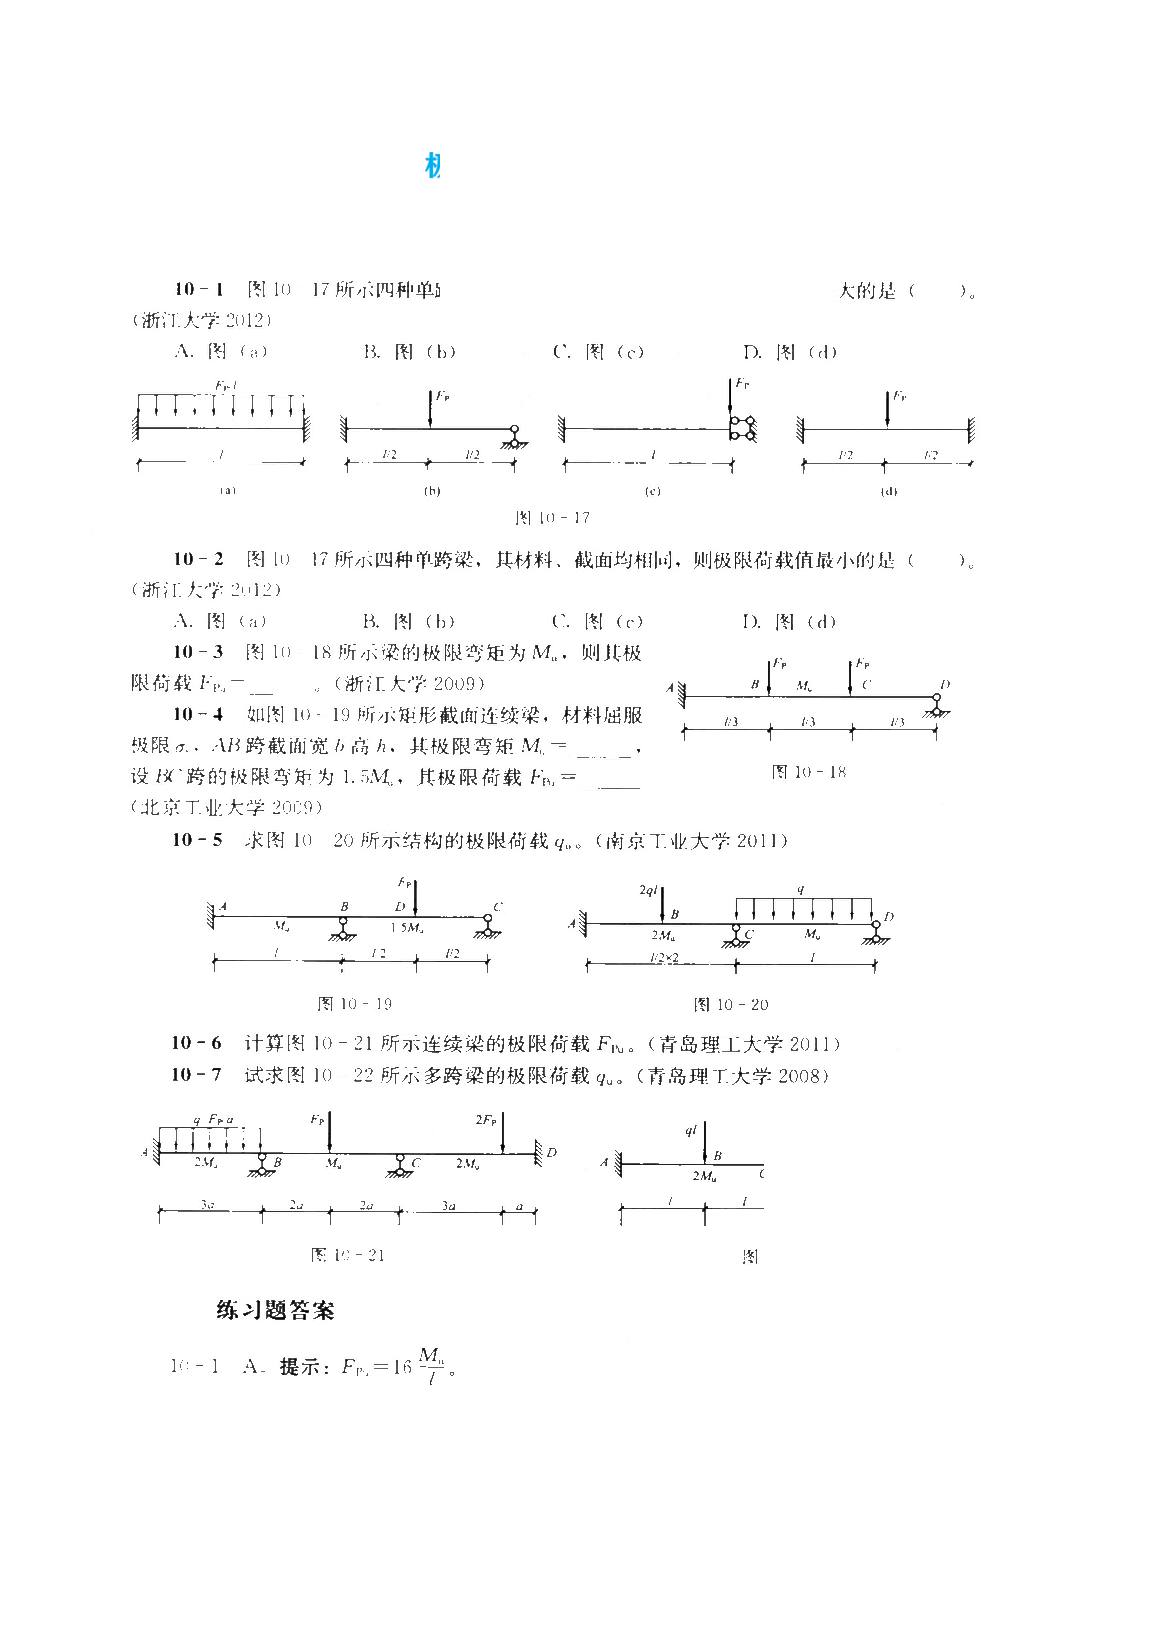
\includegraphics[width=0.92\textwidth]{figures/src20_p001.jpg}
\caption{结构力学基础与技巧班第17次作业及答案（极限荷载） 第 1 页清理图形页}
\end{figure}
\subsection*{第 2 页转写}
M.

10-2C。提示：Fpu=2

破坏时两端截面出现塑性铰。图10-17（b）Fpu=

，图10-17（d）Fpu=8

M.

M.

10-3

提示：相应的破坏机构为截面A、C出现塑性铰。

10-4

bh?

10-5

提示：相应的破坏机构为截面A、B、C出现塑性铰。

12.

Fp=2 M

10-6

提示：BC跨形成机构。

10 -7

，提示：相应的破坏机构为截面A、B、C出现塑性铰。
\begin{figure}[H]\centering
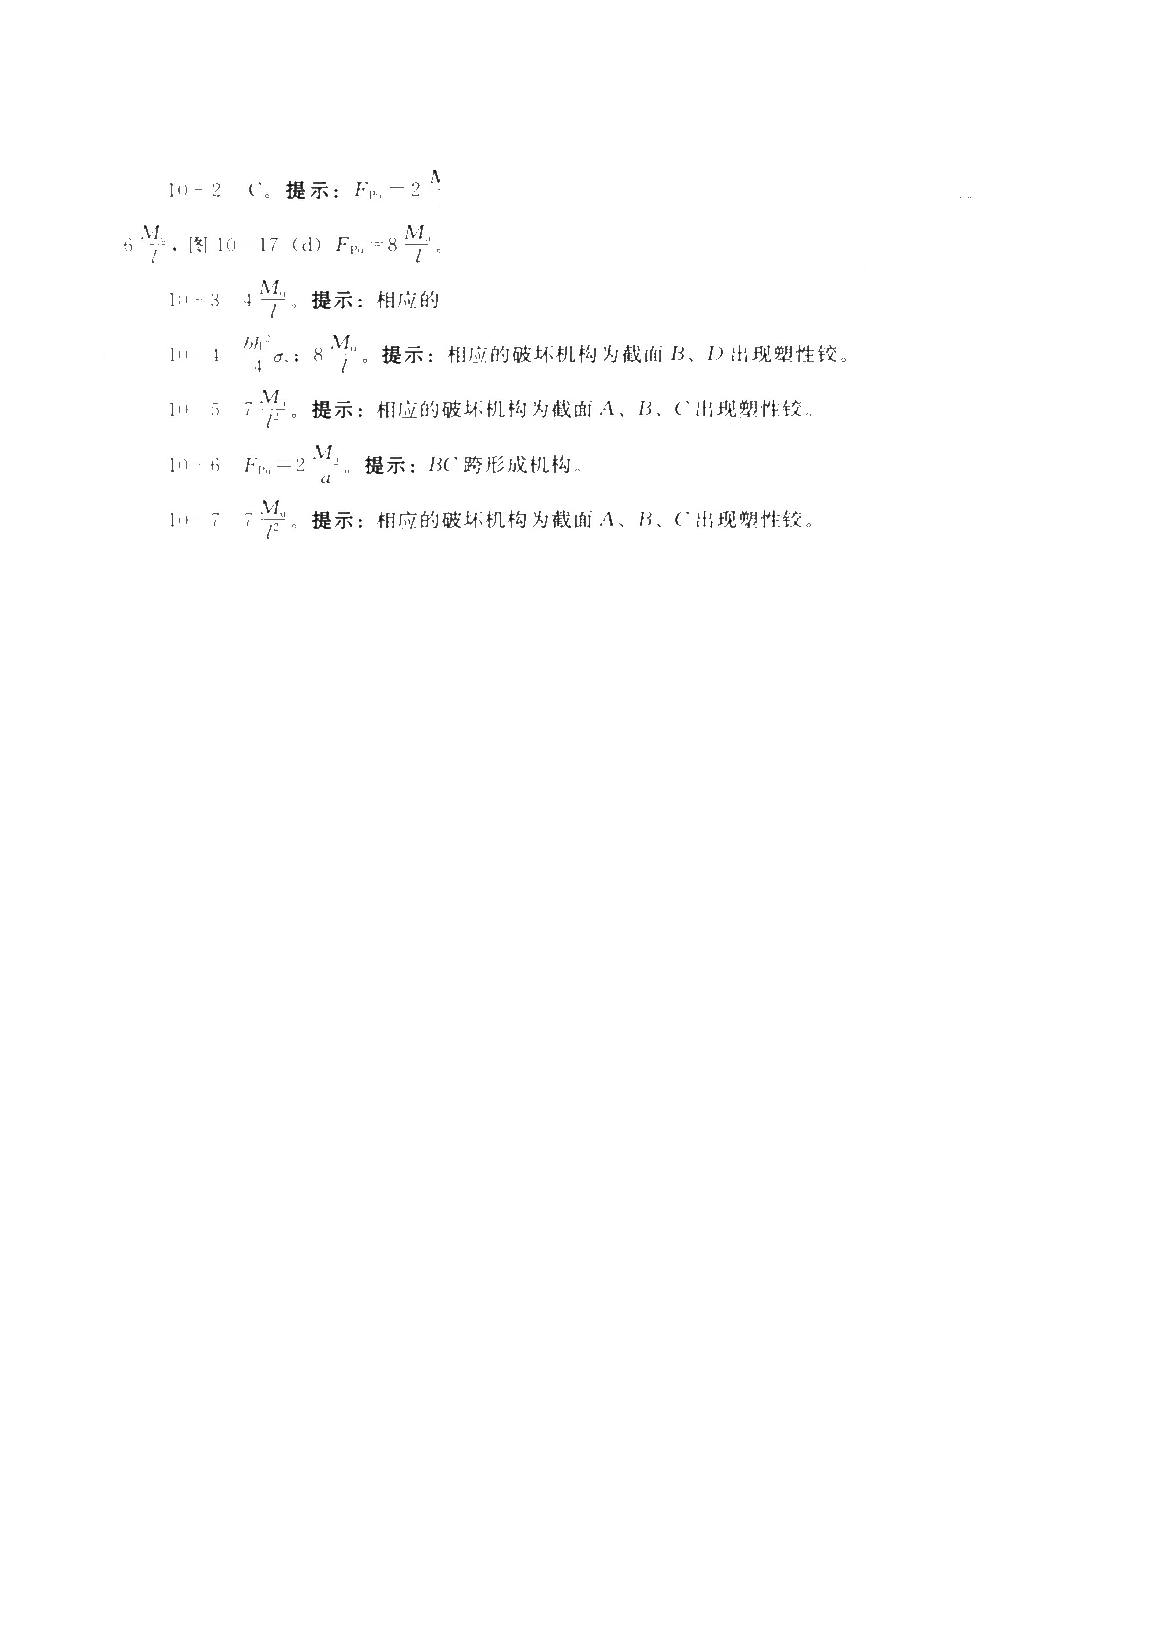
\includegraphics[width=0.92\textwidth]{figures/src20_p002.jpg}
\caption{结构力学基础与技巧班第17次作业及答案（极限荷载） 第 2 页清理图形页}
\end{figure}
\subsection*{第 3 页转写}
Mu.19+Mu19+M.29=

4Mu

bMutMu.W=Fp(0

=0mwt

Mur0+ Mu-0=p.191

=on-nw +o-nw +ony

[02、

Mu-39=

=6nw+
\begin{figure}[H]\centering
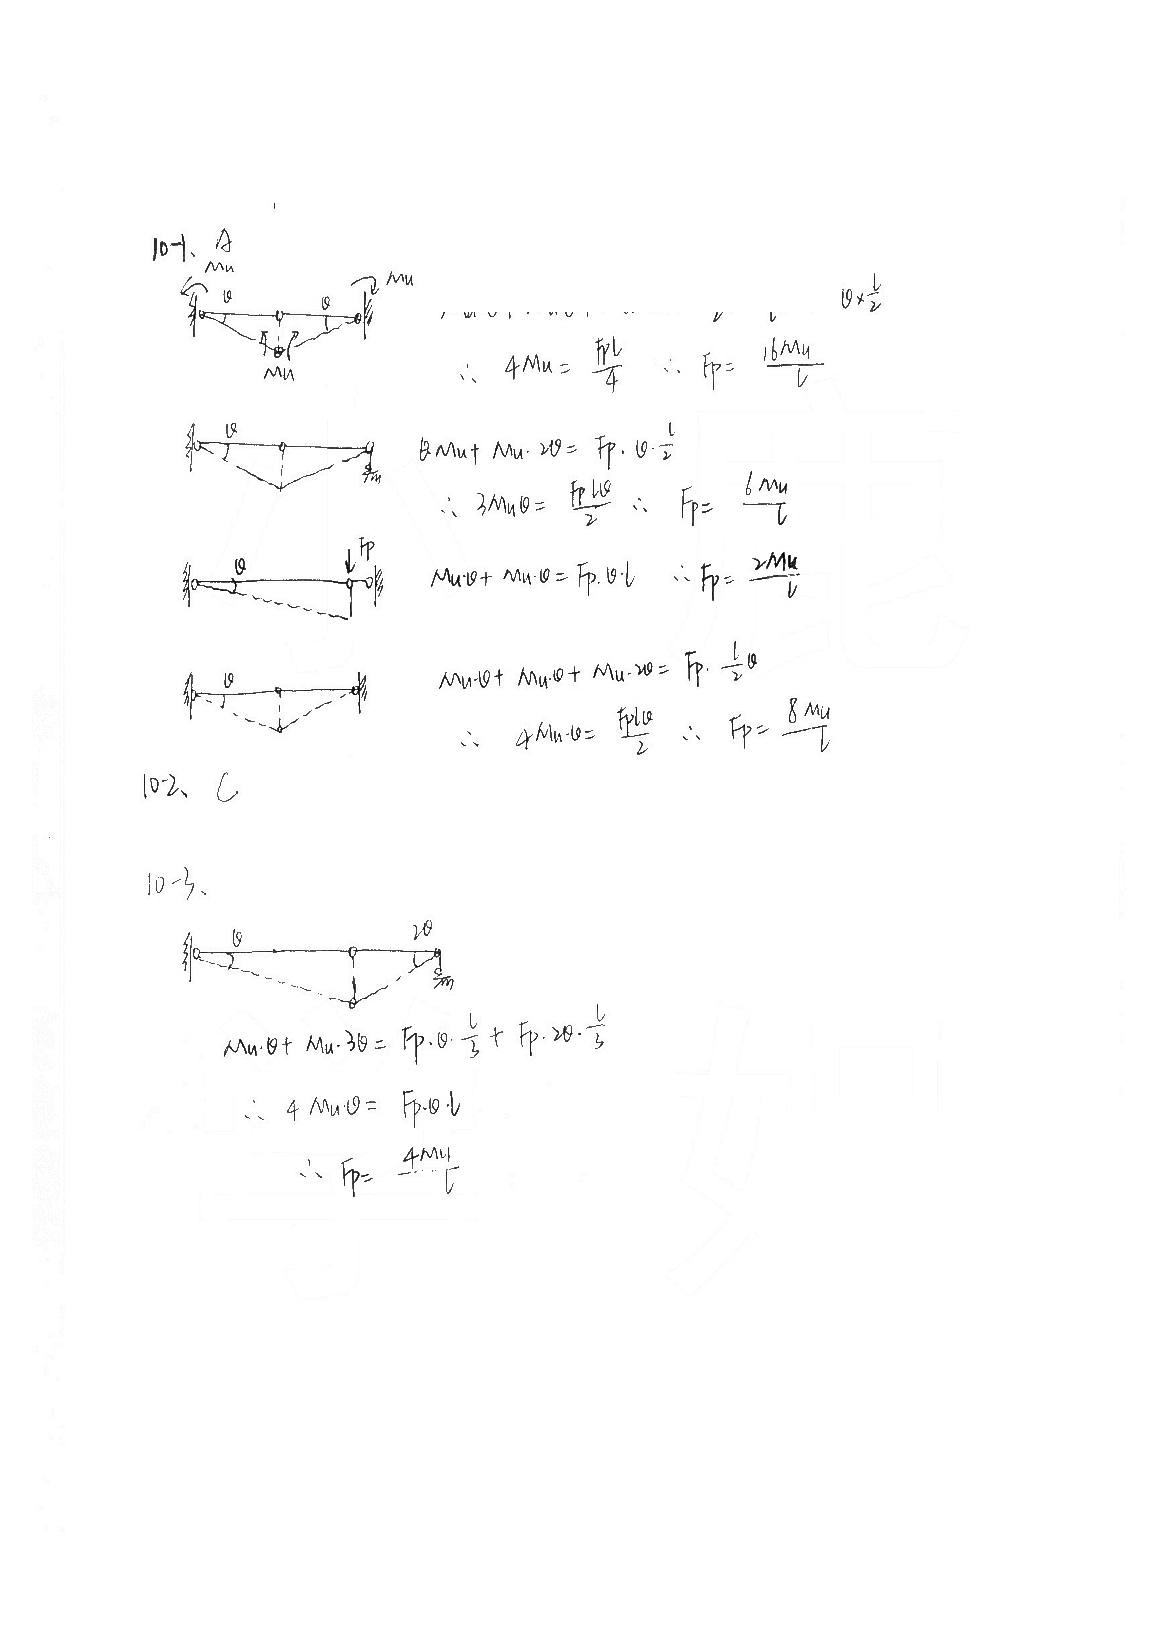
\includegraphics[width=0.92\textwidth]{figures/src20_p003.jpg}
\caption{结构力学基础与技巧班第17次作业及答案（极限荷载） 第 3 页清理图形页}
\end{figure}
\subsection*{第 4 页转写}
Mu

Mu0+15Ma.2=

4Mu-9=

8 My

= ony +on-nwn + ohwn

My

0M =0-hwL

Mu-0it Mn-(9+0\textasciitilde{})

[x9]

u (9+ 191+0)

2 Mu ((91+92+90)

X.9

(x)
\begin{figure}[H]\centering
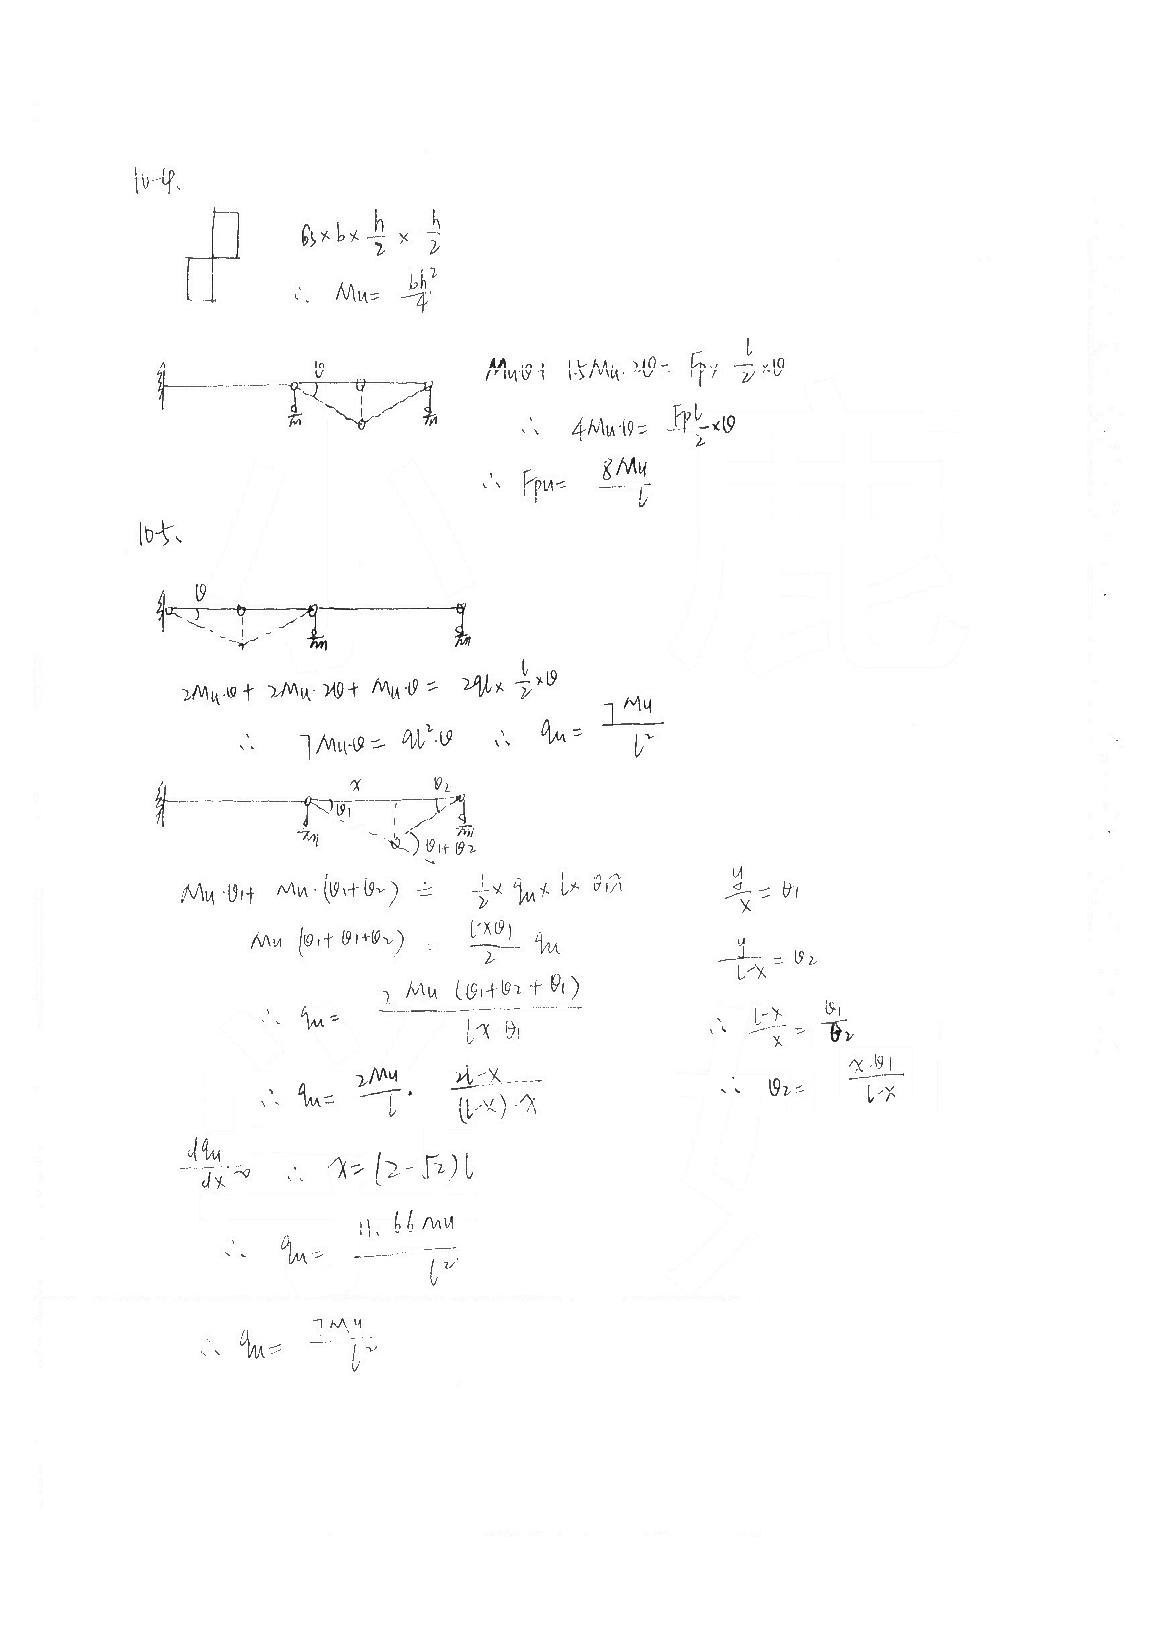
\includegraphics[width=0.92\textwidth]{figures/src20_p004.jpg}
\caption{结构力学基础与技巧班第17次作业及答案（极限荷载） 第 4 页清理图形页}
\end{figure}
\subsection*{第 5 页转写}
Mu-0+M+Mu-=

Fpx19x20

4mu9= 20xpxs

30-9

hw'si

60

3X91

2191t102+01+210\%)-

2u (40(+30)

3X91

Mul4191+310m)=

3X9

3-x

Mu

X+24ax-36

X-124

zMu

= 1614
\begin{figure}[H]\centering
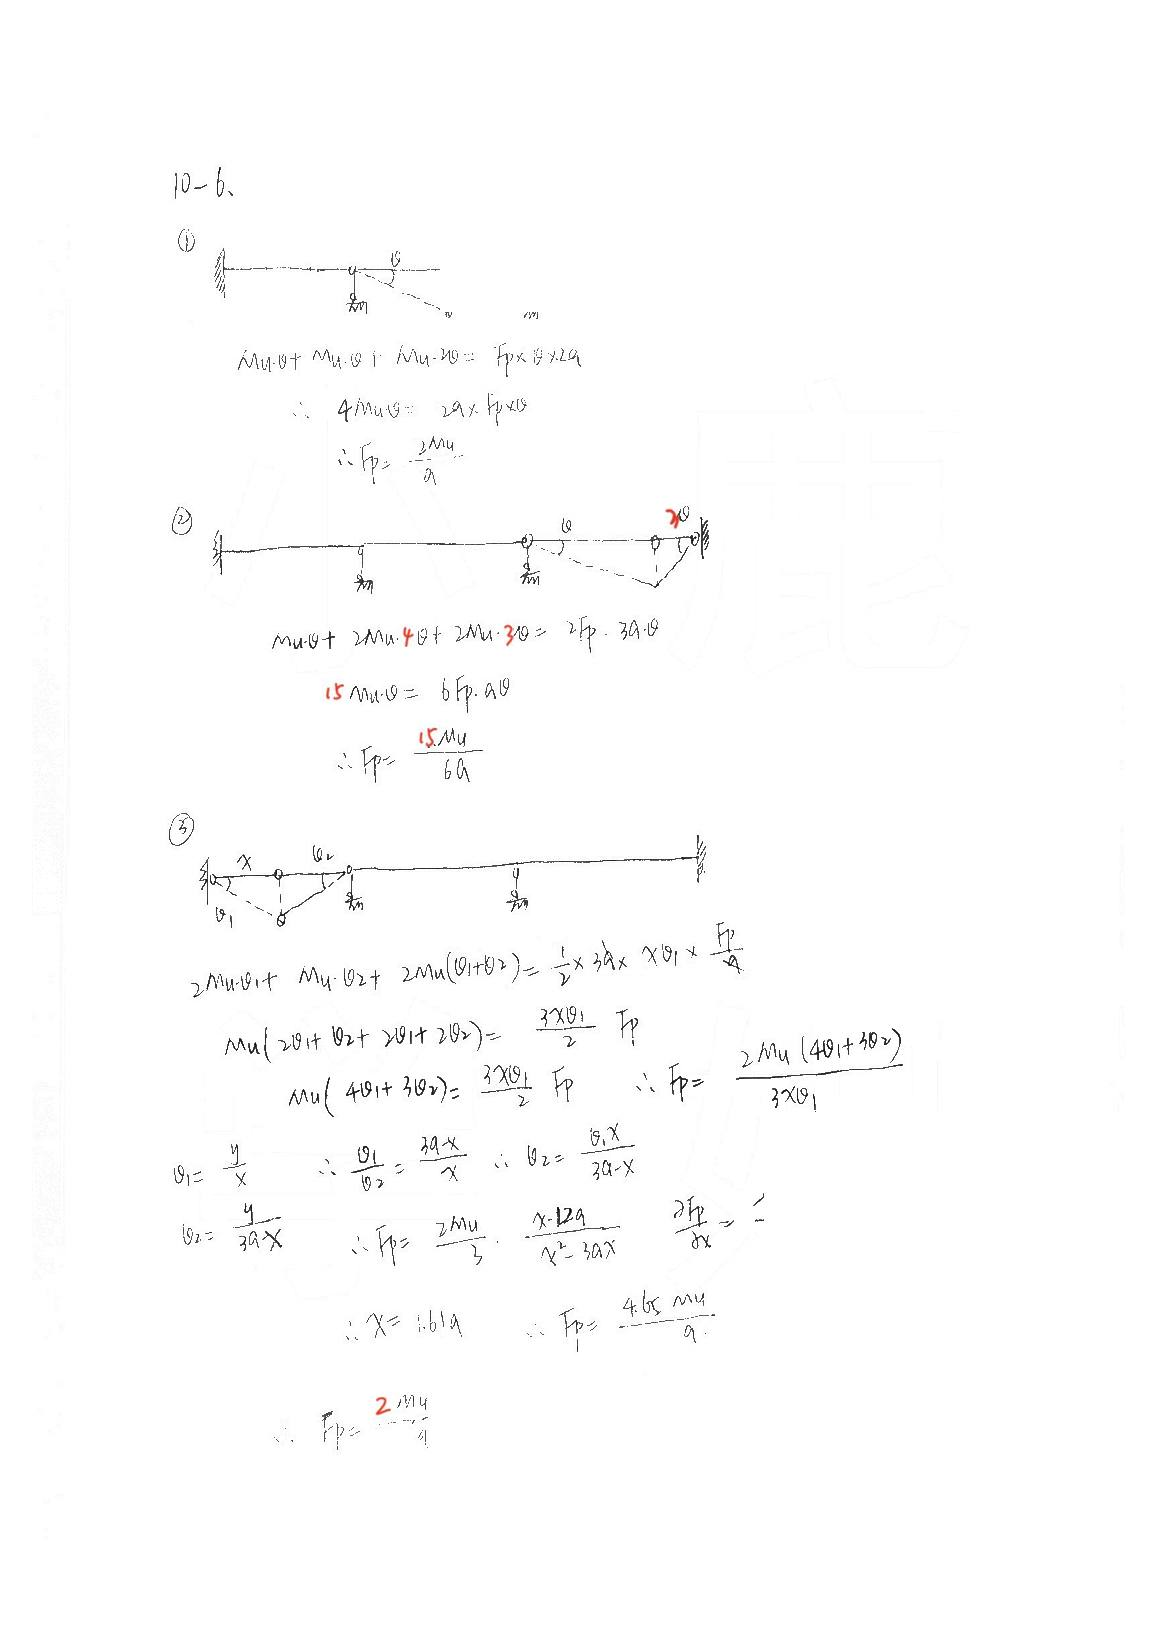
\includegraphics[width=0.92\textwidth]{figures/src20_p005.jpg}
\caption{结构力学基础与技巧班第17次作业及答案（极限荷载） 第 5 页清理图形页}
\end{figure}
\subsection*{第 6 页转写}
Imy

$\times$ =(a0+) nw7

4Mu (91t0v)

t-x

Mu19itmu-(0itloy)

Mu

2101(9)

dx

Lo1X

11.66 mu
\begin{figure}[H]\centering
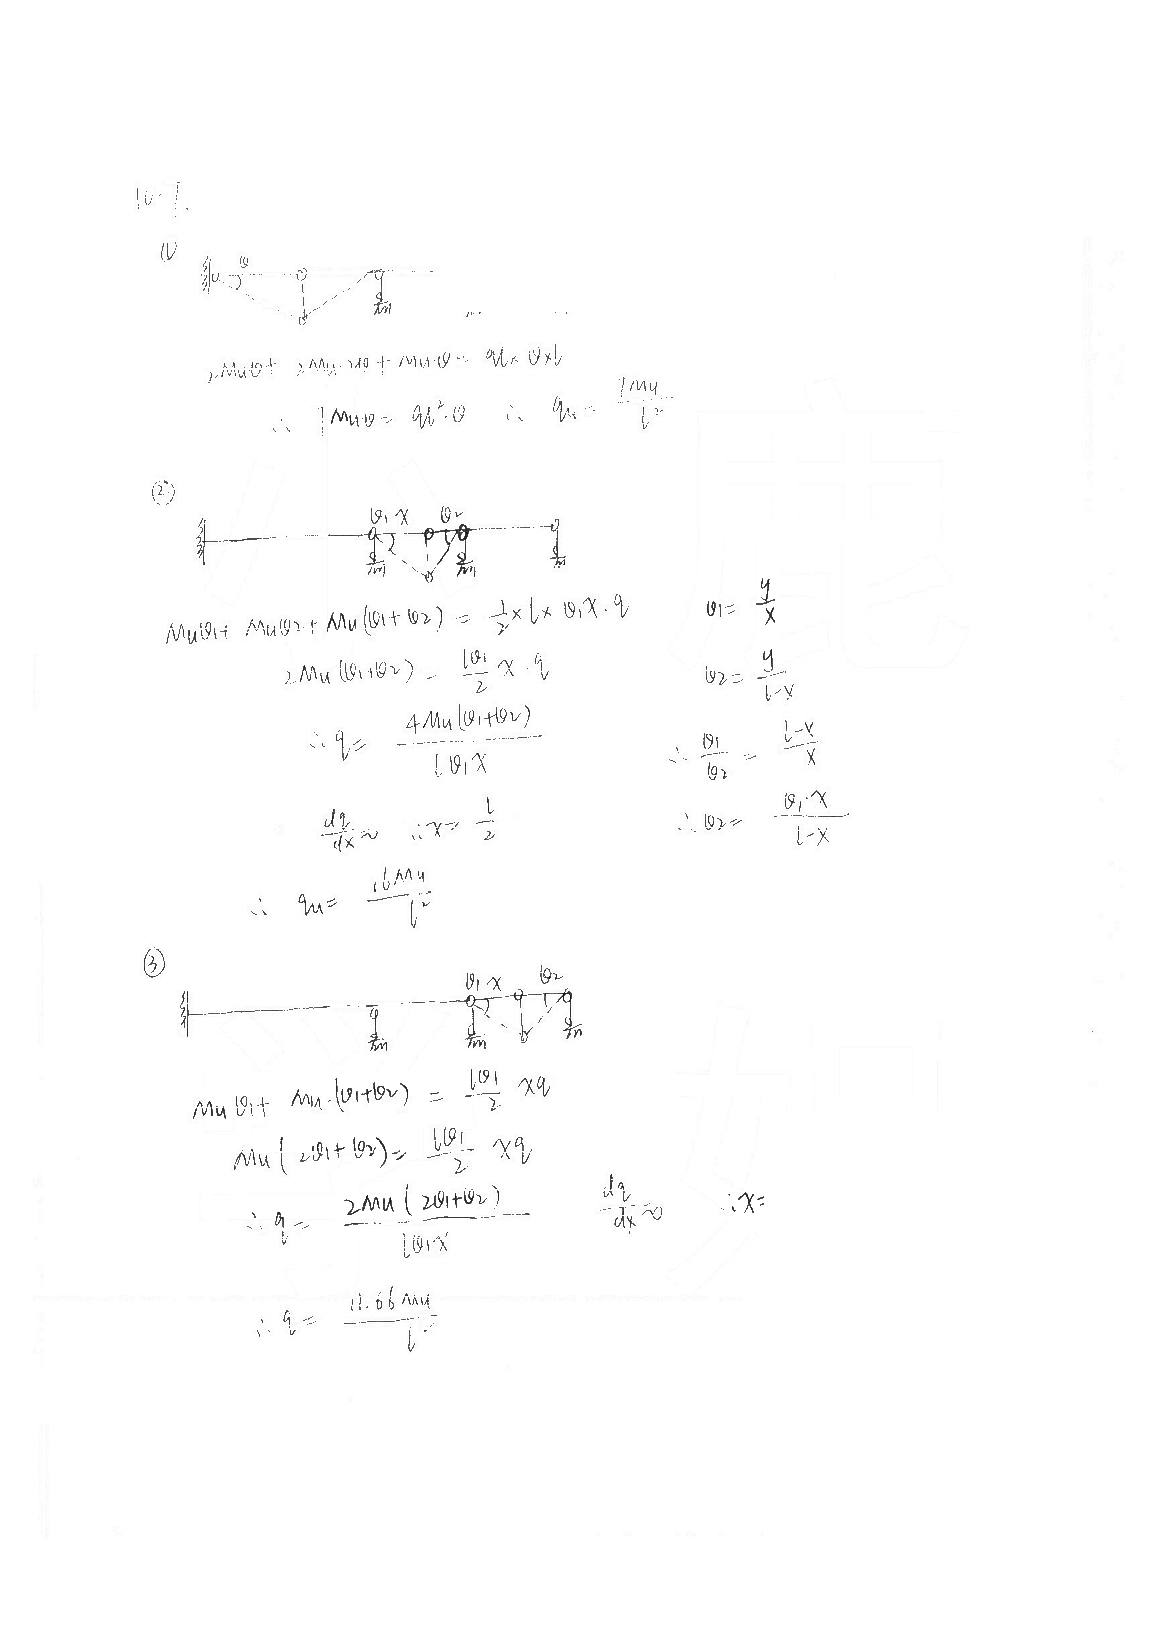
\includegraphics[width=0.92\textwidth]{figures/src20_p006.jpg}
\caption{结构力学基础与技巧班第17次作业及答案（极限荷载） 第 6 页清理图形页}
\end{figure}
